\documentclass[12pt,twoside,slovak,a4paper]{article}
\usepackage[
  top=1in,
  bottom=1in,
  left=1.25in,  % Zmenil som ľavý okraj na 1.25in
  right=1.25in, % Zmenil som pravý okraj na 1.25in
]{geometry}

\usepackage[slovak]{babel}
\usepackage[T1]{fontenc}
\usepackage[utf8]{inputenc}
\usepackage{lmodern} % moderný font
\usepackage{microtype} % zlepšenie sadzby
\usepackage{graphicx}
\usepackage{url}
\usepackage{hyperref}
\usepackage{titlesec} % prispôsobenie nadpisov
\usepackage{booktabs} % pre peknejšie tabuľky
\usepackage{cleveref} % inteligentné referencie
\usepackage{indentfirst} % zarezávanie prvého riadku po nadpise
\usepackage{float} % Ku tabulke
\usepackage{booktabs} %pekny styl tabulky
\usepackage{adjustbox}


\title{Ako algoritmy sociálnych médií získavajú informácie 
z používateľov a následne ich využívajú vo svoj 
prospech}

\author{David Vach\\
	{\small Slovenská technická univerzita v Bratislave}\\
	{\small Fakulta informatiky a informačných technológií}\\
	{\small \texttt{xvachd@stuba.sk}}\\
	{\small Vedenie: Mirwais Ahmadzai}
}

\date{\small 16. december 2023} 

% Definície štýlov nadpisov
\titleformat{\section}
  {\normalfont\Large\bfseries}
  {\thesection}{2em}{}

\titleformat{\subsection}
  {\normalfont\large\bfseries}
  {\thesubsection}{1em}{}

% Vlastné definície pre abstract a kľúčové slová
\newcommand{\keywords}[1]{
  \small	
  \textbf{\textit{Kľúčové slová---}} #1
}

\begin{document}

\maketitle

\begin{abstract}
Tento článok sa bude venovať podrobnej analýze získavaniu informácii používateľov sociálnych médií pomocou algoritmov. Práca bude pozostávať z toho ako sa tieto algoritmy snažia získať čo najviac informácií z používateľov, ktoré následne môžu využiť na rôzne marketingové ciele. Jadro tohto článku sa sústreďuje na algoritmy a ich efektivite v udržiavaní pozornosti používateľov na základe získaných dát a následné zobrazovanie špecifického obsahu za účelom získať čo najviac presnejších dát a následné vymazávanie nepotrebných dát. Ďalšia časť tejto práce ukazuje rôzne spôsoby zneužívania týchto dát vo svoj prospech z dlhodobého hľadiska a ako tieto algoritmy vedia pomocou získaných dát určiť s veľkou pravdepodobnosťou osobnosť používateľa a iné citlivé informácie. Záver práce tvoria dôvody prečo by sme si mali tieto súkromné dáta chrániť a aké spôsoby sa na to využívajú.
\end{abstract}

\keywords{sociálne médiá, zber dát, ochrana súkromia, algoritmy, marketing}

\newpage
\section{Úvod}


V úvode dnešnej digitálnej éry predstavujú sociálne médiá viac než len platformy na zdieľanie osobných príbehov a fotografií. Sú to sofistikované ekosystémy využívajúce algoritmy, ktoré transformujú spôsob, akým komunikujeme, angažujeme sa a dokonca ako sa rozhodujeme. Algoritmy sociálnych médií sú navrhnuté tak, aby boli nenápadnými, no mocnými kustódmi našej online pozornosti.

Tieto algoritmy pracujú na základe predpokladu, že každá interakcia na platforme - lajk, zdieľanie, komentár, dokonca aj dĺžka zdržania sa pri príspevku - je cenným údajom, ktorý odhaľuje náš vkus, preferencie a správanie. Tieto údaje sú potom analyzované a transformované na mieru, ktorá nás drží zapojených – a často prilepených – na naše obrazovky dlhšie než sme plánovali.

No táto personalizácia má aj svoju cenu. Algoritmy sociálnych médií sú takisto navrhnuté na podporu obchodných modelov ich prevádzkovateľov, čo znamená, že informácie získané z používateľských interakcií sú často využívané na cieľovú reklamu a obsahové odporúčania, ktoré podporujú angažovanosť a zisky. Tento proces môže používateľov nevedomky manipulovať k tomu, aby konzumovali obsah a produkty, ktoré možno nepotrebujú alebo dokonca nechcú.

Jedným z hlavných problémov týchto algoritmov je ich neschopnosť porozumieť ironii a sarkazmu. To vedie k tomu, že dáta, ktoré tieto algoritmy vyprodukuju, môžu obsahovať nepresné informácie a interpretácie. Používatelia často využívajú ironiu a sarkazmus vo svojich príspevkoch na sociálnych médiách, čo môže algoritmy zmiasť a viesť k nesprávnym záverom.

Tento úvod bude skúmať, ako algoritmy sociálnych médií zbierajú a využívajú používateľské informácie a aké sú implikácie tohto procesu na súkromie, spoločenské správanie a dokonca na demokraciu. Dôležitou témou bude aj vplyv týchto algoritmov na manipuláciu s používateľmi a formovanie ich názorov prostredníctvom personalizovaného obsahu a reklamy.

Na záver, bude sa táto práca venovať aj možnostiam riešenia tohto problému a zlepšeniu efektívnosti algoritmov sociálnych médií v interpretácii komplexných používateľských prejavov vrátane ironie a sarkazmu.
\cite{7087040} \cite{7783248}


\section{Súvisiaca práca}


V tejto sekcií sa venujeme prehľadu literatúry, ktorá sa zaoberá rôznymi aspektmi analýzy a klasifikácie dát sociálnych médií, ako aj predpovedaním a vizualizáciou spotrebiteľských nálad. Táto analýza literatúry nám pomôže lepšie pochopiť komplexnosť a rôznorodosť prístupov k riešeniu problémov spojených so sociálnymi médiami.

Zhang et al. \cite{7809906} sa zameriavajú na predpovedanie a vizualizáciu spotrebiteľských sentimentov v online sociálnych médiách. Tento prístup je dôležitý pre pochopenie správania sa spotrebiteľov a ich postojov voči rôznym produktom a službám.

Desai a Patil \cite{7087040} skúmajú efektívne regresné algoritmy pre klasifikáciu dát sociálnych médií. Ich práca poskytuje užitočné informácie o tom, ako efektívne spracovať a analyzovať veľké množstvá dát.

Reddy a Parvathy \cite{9952138}, ako aj Reddy a Kumar \cite{9952143}, poskytujú inovatívne metódy na predpovedanie úrovne znečistenia ovzdušia, resp. na určovanie presnosti cien akcií s využitím algoritmov náhodných lesov a gradient boosting.

Rizky Pribadi et al. \cite{10057722} sa zameriavajú na analýzu angažovanosti používateľov sociálnych médií na trhoviskách podľa tém, čo je kľúčové pre marketing a reklamu.

Shahare \cite{8250692} sa venuje analýze sentimentu pre dáta z novín na základe sociálnych médií, čo je dôležité pre pochopenie verejnej mienky a trendov.

Zhang et al. \cite{8575882} a Zhang \cite{9719080} skúmajú výber funkcií a algoritmy učenia založené na hlbokých neurónových sieťach pre dáta zo sociálnych médií, čo je dôležité pre efektívne spracovanie a analýzu týchto dát.

Arambepola a Munasinghe \cite{9325452} sa zameriavajú na empirickú analýzu faktorov používateľov ovplyvňujúcich dizajn používateľského rozhrania v mobilných aplikáciách, čo je dôležité pre optimalizáciu používateľského zážitku.

Rohani et al. \cite{7783248} poskytujú praktický prístup k modelovaniu tém pre obsah sociálnych médií, čo je kľúčové pre porozumenie a analyzovanie diskusií a trendov na sociálnych sieťach.

Napokon, Fan et al. \cite{1250902} sa zaoberajú otázkou, či je náhodný model lepší z hľadiska presnosti a efektívnosti, čo je zásadný príspevok k diskusii o optimálnych modeloch pre dáta sociálnych médií. Táto sekcia nám ukazuje rozmanitosť výskumu v oblasti analýzy sociálnych médií a jeho dôležitosť pre rôzne odvetvia vrátane marketingu, financií a verejnej mienky.

\section{Metodológia}

V rámci tejto štúdie sme sa zameriavali na analýzu algoritmov sociálnych médií a ich vplyvu na správanie používateľov. Naša metodológia zahŕňala niekoľko dôležitých krokov.

Prvým krokom bolo výber relevantných dátových sád zo sociálnych médií, pričom sme sa špecifickejšie zameriavali na obdobie posledných dvoch rokov. Tieto dáta zahŕňali rôzne používateľské interakcie, ako sú lajky, komentáre a zdieľanie obsahu.

Následne sme prešli k analýze konkrétnych algoritmov používaných na týchto platformách, vrátane algoritmov ako NaiveBayes a Adaboost. Našim cieľom bolo posúdiť ich efektivitu v personalizácii obsahu a skúmať, aký vplyv majú na používateľské správanie.

Pri analýze dát sme využívali techniky spracovania prirodzeného jazyka a analýzy sentimentu, aby sme získali hlbší pohľad na povahu týchto dát. Počas celého procesu sme venovali osobitnú pozornosť etickým aspektom spojeným so zberom a analýzou používateľských dát.

Na vyhodnotenie účinnosti rôznych algoritmov sme použili špecifické metriky, ako sú miera zapojenia používateľov a čas strávený na platforme. Táto metodológia nám umožnila poskytnúť podrobnejšie pochopenie toho, ako algoritmy sociálnych médií ovplyvňujú používateľské správanie a súkromie.


\section{Ako tieto algoritmy fungujú}
Algoritmy sociálnych médií sú navrhnuté tak, aby efektívne zbierali a analyzovali údaje generované užívateľmi pri ich interakciách online. Ich schopnosť poskytovať personalizovaný obsah je založená na dômyselnom sledovaní a vyhodnocovaní činností používateľov. Keď používateľ lajkuje príspevok, komentuje video alebo strávi určitý čas čítaním článku, tieto akcie sú zaznamenané a stávajú sa časťou veľkého údajového modelu, ktorý tento algoritmus používa na pochopenie a predvídanie preferencií používateľa.\cite{10057722}

Na základe textu, obrázkov a videí, ktoré používatelia zdieľajú alebo komentujú, algoritmy využívajú pokročilé metódy ako spracovanie prirodzeného jazyka a rozpoznávanie obrazu na to, aby lepšie porozumeli obsahu, ktorý používatelia preferujú. Algoritmy zároveň skúmajú vzťahy a interakcie medzi používateľmi, aby zistili, aké sociálne siete sú pre nich najdôležitejšie a ako sa tie môžu prepojiť s ich obsahovými preferenciami.

Na základe získaných dát tieto algoritmy vytvoria obsah, ktorý sa používateľom zobrazuje vo feedoch, aby bol čo najrelevantnejší a najzaujímavejší. Tento personalizovaný prístup sa nezameriava len na zvýšenie užívateľskej spokojnosti a zapojenia, ale je tiež základom pre efektívnu cieľovú reklamu, kde sú reklamy prispôsobené konkrétnym záujmom a správaniu používateľov.

Súčasťou procesu je aj predpovedanie správania. Algoritmy sociálnych médií sa pokúšajú predvídať, čo by mohlo používateľov zaujímať v budúcnosti, a prispôsobujú svoje stratégie, aby bol obsah, ktorý zobrazujú, vždy krok vpred. Vďaka neustálej spätnej väzbe a iterácii sa algoritmy neustále učia a zdokonaľujú, aby boli ešte lepšie v predvídavaní a napĺňaní očakávaní užívateľov.


Názorný príklad pre Facebook:

\begin{figure}[h]
    \centering
    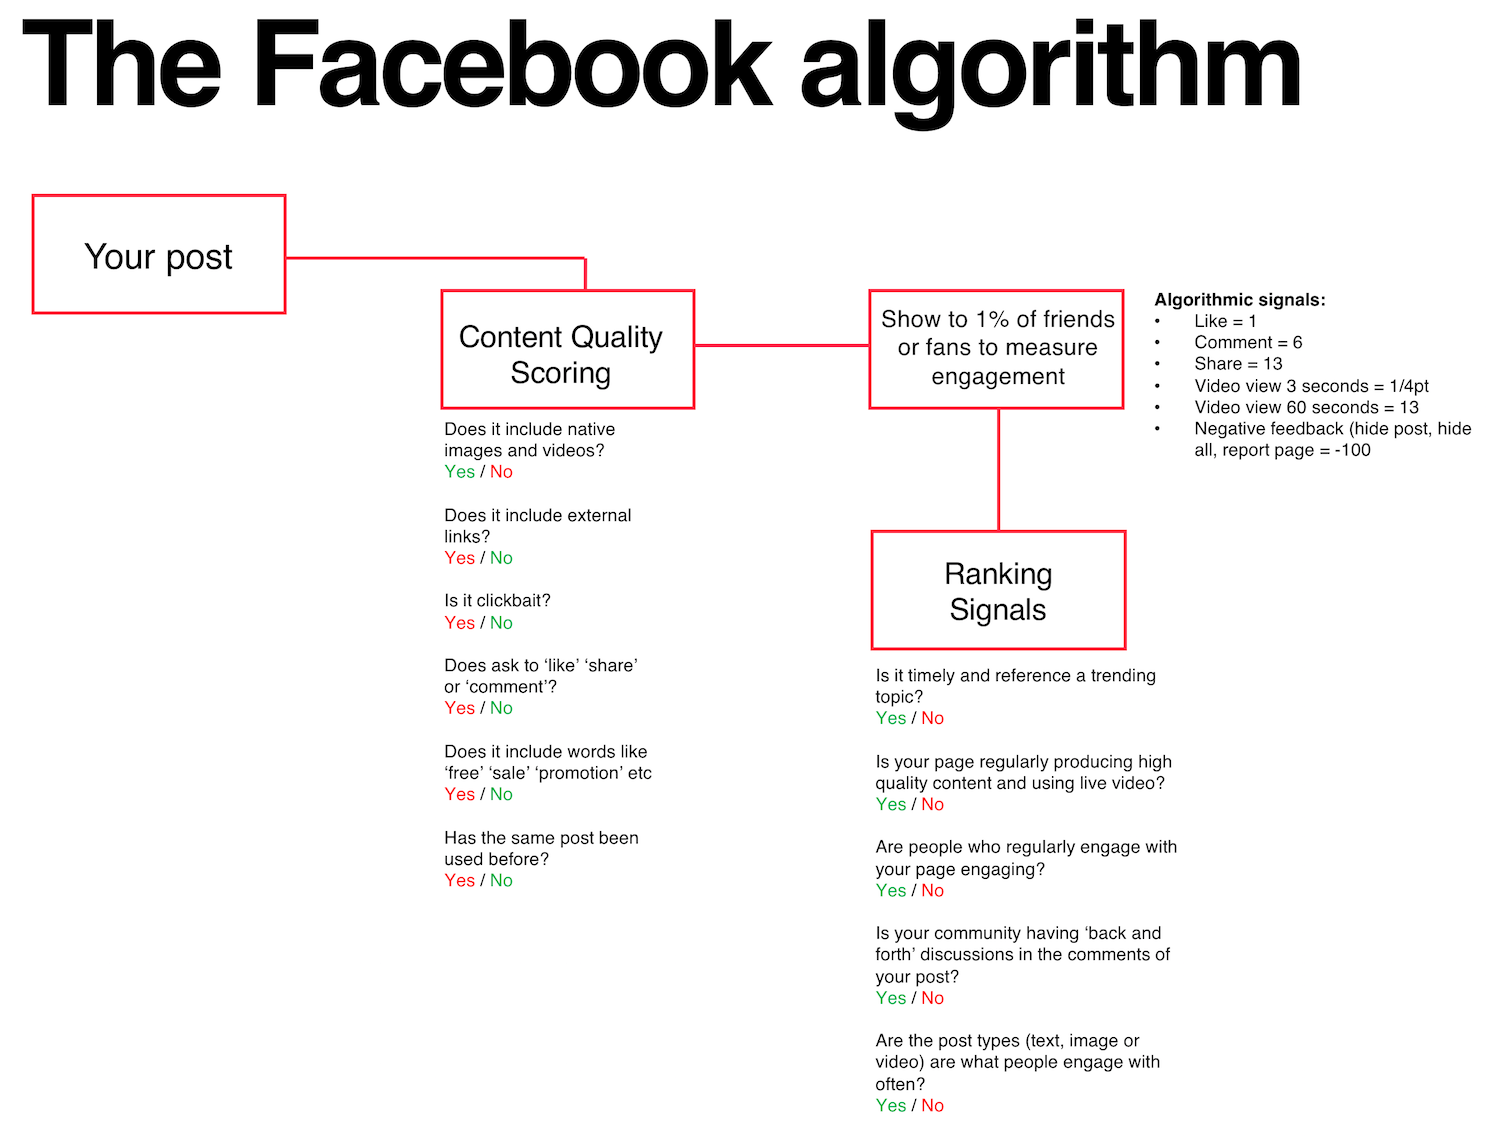
\includegraphics[scale=0.6]{FacebookAlgorithmExample.PNG} 
    \caption{Truncation of SVD for LSI. \cite{7087040}} % sem pridaj citaciu
    \label{fig:truncation}
\end{figure}


Výsledkom je, že algoritmy sociálnych médií tvoria dynamický a neustále sa vyvíjajúci systém, ktorý je mimoriadne citlivý na potreby a chovanie používateľov, a to všetko v úsilí udržať ich zapojenie a poskytnúť im maximálne prispôsobený zážitok. Ekonomický model sociálnych sietí, založený predovšetkým na reklamných príjmoch, je priamo ovplyvnený úspešnosťou týchto algoritmov v predpovedaní a ovplyvňovaní používateľského správania.








\section{Analýza}
Analýza algoritmov strojového učenia v kontexte sociálnych médií je kľúčovou časťou našej štúdie. Tieto algoritmy majú zásadný vplyv na to, ako sú prezentované informácie používateľom a ako sú tieto informácie personalizované. Na túto analýzu sme vybrali viacero algoritmov strojového učenia, ktoré budeme dôkladne analyzovať z hľadiska ich výhod, nevýhod a najlepších použití.



\subsection{NaiveBayes\cite{7809906}}

\subsection{Adaboost\cite{7087040}}

\subsection{Random Forest\cite{9952138}}

\subsection{Gradient Boosting Machines (GBM)\cite{9952143}}




\begin{table}[h]
\centering
\begin{tabular}{|l|p{4cm}|p{4cm}|p{3cm}|}
\hline
\textbf{Algoritmus} & \textbf{Výhody} & \textbf{Nevýhody} & \textbf{Najlepšie použitie} \\
\hline
Adaboost & Zlepšuje slabé modely, prispôsobivý & Citlivý na šum, náchylný na preučenie & Klasifikácia 'náročných' prípadov \\
\hline
NaiveBayes & Jednoduchý, rýchly, efektívny pre textové dáta & Predpokladá nezávislosť atribútov, môže byť menej presný & Klasifikácia textu, filtrovanie spamu \\
\hline
GBM & Vysoká presnosť, efektívny pre komplexné vzory & Náchylný na preučenie, výpočtovo náročný & Klasifikácia a regresia s komplexnými vzormi \\
\hline
Random Forest & Odolný voči preučeniu, efektívny pre veľké dáta & Menej interpretabilný, výpočtovo náročný & Klasifikácia a regresia, veľké dáta \\
\hline
\end{tabular}
\caption{Porovnanie algoritmov strojového učenia podľa článku Desai a Patil \cite{7087040} a ďalších prác \cite{7809906,9952138,9952143}}
\label{table:algorithm_comparison}
\end{table}



\section{Výsledok}


\section{Záver} 

V závere našej štúdie sme dospeli k dôležitým zisteniam týkajúcim sa algoritmov sociálnych médií a ich vplyvu na používateľov. Naše analýzy ukázali, že tieto algoritmy hrajú kľúčovú úlohu v personalizácii obsahu a vytváraní zapojenia používateľov. Sú schopné efektívne zbierať, analyzovať a predvídať používateľské preferencie na základe ich interakcií na platformách sociálnych médií.

S týmto prispôsobovaním však prichádza aj riziko zneužitia a narušenia súkromia používateľov. Algoritmy môžu byť zneužité na manipuláciu s používateľskými správaniami a na cieľovú reklamu, ktorá niekedy prekračuje hranice etiky. Je preto nevyhnutné, aby sa vývoj a implementácia týchto algoritmov riadila prísnymi etickými normami a normami týkajúcimi sa ochrany súkromia.

Transparentnosť a regulácia v oblasti algoritmov sociálnych médií sú kľúčovými faktormi na zaistenie bezpečnosti a súkromia používateľov. Je dôležité, aby platformy sociálnych médií aktívne pracovali na zlepšovaní svojich algoritmov a na ochrane súkromia svojich používateľov.

Celkovo nás naša štúdia núti zamyslieť sa nad tým, ako sú naše údaje spracovávané a využívané na sociálnych médiách, a zdôrazňuje potrebu ochrany súkromia a etického využívania algoritmov. Len tak môžeme zabezpečiť, že budúcnosť sociálnych médií bude prospešná a bezpečná pre všetkých používateľov.




\section{Reakcia na prednášky}

\subsection{Kreatívne písanie (Prednáška 8)}

Kreatívne písanie je umenie, ktoré umožňuje autorom vyjadriť svoje myšlienky, emócie a predstavy prostredníctvom slov. Je to proces, ktorý spočíva v tvorbe originálnych textov, či už ide o poéziu, prózu, drámu alebo iné literárne formy. Pri kreatívnom písaní je dôležitá nielen schopnosť gramaticky správneho a zrozumiteľného vyjadrovania, ale predovšetkým originalita a kreativita. Autor by mal byť schopný preniesť čitateľa do svojho sveta, ukázať mu nové perspektívy a vyvolať v ňom emócie.

Kľúčom k úspechu v kreatívnom písaní je pravidelná prax a ochota experimentovať so slovami a štýlom. Dobrý autor by mal byť otvorený novým nápadom a neprestajne rozvíjať svoje písacie zručnosti. Kreatívne písanie nie je len o výroku umeleckých diel, ale aj o sebavyjadrení a osobnom rozvoji. Táto forma písania môže byť terapeutická a umožňuje autorom vyrovnať sa s osobnými záležitosťami alebo spracovať svoje myšlienky a pocity. Preto je dôležité vytvárať prostredie, kde sa autori cítia inšpirovaní a majú priestor na kreativitu.

\subsection{Plagiátorstvo (Prednáška 9)}
Plagiátorstvo je téma, o ktorej by mal byť každý tvorca článku, eseje, prezentácie alebo autor akéhokoľvek verejného prejavu oboznámený. Dá sa to nazvať krádežou, ale niekedy sa môže človek dopustiť neúmyselnému plagiátorstvu. Spôsob, akým sa mu vyhnúť je jednoduchý, a to odkazovať sa na použité zdroje.

\subsection{Technológia a ľudia: Scrum. doc. Valentino Vranić (Prednáška 11)}
Scrum predstavuje cenný nástroj aj v akademickom prostredí. Pre mňa osobne znamená efektívny spôsob organizácie a riadenia mojich študijných projektov a úloh. Princípy Scrumu, ako je rozdelenie práce do krátkych iterácií a pravidelné kontroly, mi pomáhajú udržať si prehľad nad rozsiahlymi úlohami. Zahrnutie flexibility na reagovanie na nečakané zmeny v pláne mi umožňuje byť pripravený na všetko, čo sa počas semestra môže stať.

Okrem toho, Scrum podporuje silnú spoluprácu tímu, čo je dôležité v rámci skupinových projektov a prezentácií. Dokážeme lepšie komunikovať, sledovať postup jednotlivých členov tímu a včas identifikovať prípadné problémy. Týmto spôsobom sa stávame efektívnejšími a dosahujeme lepšie výsledky.


%POZNAMKA K TEJTO SEKCII
%1.
% It is not recommended to include the title of the article in
%the related work section. Instead, provide a brief summary of %the main
%focus of the article in one or two sentences.


%2. Student contribution and research methodology are missing in the
%article.
%
%3. The first lengthy paragraph in the introduction section lacks
%professional structure; consider breaking it down into sub-paragraphs.
%
%4. The first paragraph in the introduction lacks citations, making it
%unclear whether the ideas presented are the student's or from other
%sources.
%
%5. Ensure that reference numbers are in ascending order, and correct the
%"?" mark in some citations, such as the one in the diagram





%LITERATURA
\nocite{10057722}
\nocite{7087040}
\nocite{7783248}
\nocite{7809906}
\nocite{8250692}
\nocite{8575882}
\nocite{9325452}
\nocite{9719080}
\nocite{9952138}
\nocite{9952143}
\nocite{1250902}
\nocite{6616536}

\bibliographystyle{abbrv}
\bibliography{bibtex}

%KONIEC DOKUMENTU
\end{document}